% for slides
\documentclass{beamer}

% for 1 page per slide printouts
% \documentclass[handout]{beamer}
% \usepackage{pgfpages}
% \pgfpagesuselayout{resize to}[a4paper,landscape,border shrink=5mm]

%\documentclass[handout]{beamer}
%\usepackage{pgfpages}
%\pgfpagesuselayout{4 on 1}[a4paper,landscape,border shrink=5mm]

% \documentclass[handout]{beamer}
% \usepackage{pgfpages}
% \pgfpagesuselayout{2 on 1}[a4paper,border shrink=5mm]

% set to show the notes made throughout as slides
% best used in the 2on1 handouts for reference by speaker
% \setbeameroption{show notes}

\usepackage{oz}
\usepackage{multicol}
\usepackage{multimedia}
\usepackage{mathtools}

\newcommand{\Poincare}{Poincar\'{e}}
\newcommand{\Complex}{\mathbb{C}}
\newcommand{\Rpart}[1]{\mathfrak{R}\left(#1\right)}
\newcommand{\Real}{\mathbb{R}}
\newcommand{\Rational}{\mathbb{Q}}
\newcommand{\Integer}{\mathbb{Z}}
\newcommand{\Natural}{\mathbb{N}}
\newcommand{\CP}{\mathbf{CP}}
\newcommand{\RP}{\mathbf{RP}}

\newcommand{\PTIME}{\mathbf{P}}
\newcommand{\NPTIME}{\mathbf{NP}}
\newcommand{\DTIME}{\mathbf{DTIME}}
\newcommand{\NTIME}{\mathbf{NTIME}}

\renewcommand{\vec}[1]{\mathbf{#1}}

\usetheme[progressbar=title]{metropolis}           % Use metropolis theme
\title{The Millennium Prize Problems}
\subtitle{A PGR Seminar in Two Parts}
\date{}
\author{Luke Smallman}
\institute{Cardiff University} \titlegraphic{\hfill
\includegraphics[height=1.5cm]{logo}}


\begin{document}
  \maketitle
  \begin{frame}{Structure}
      \begin{multicols}{2}
          \tableofcontents
      \end{multicols}
  \end{frame}

  \section{Introduction}
  \begin{frame}{Introduction}
      \pause
      \begin{itemize}
          \item The Millennium Prize Problems were seven unsolved problems
              set out by the Clay Mathematics Institute
      \pause
          \item The Millenium Prize Problems are now six unsolved problems
              and one solved problem.
      \pause
          \item They have a certain level of infamy due to the Clay
              Mathematics Institute's promise of \$1 million for a correct
              proof of any of the problems
      \end{itemize}
  \end{frame}

  \section{$\PTIME$ versus $\NPTIME$}
  \begin{frame}{$\PTIME$ vs $\NPTIME$}
      \begin{block}{Problem Statement}
          Prove or disprove that $\PTIME = \NPTIME$
      \end{block}
  \end{frame}
  \begin{frame}{The Deterministic Turing Machine}
      \pause
      \begin{block}{Definition}
          \pause
          \begin{table}[]
              \centering
              \begin{tabular}{ll}
                  $\Box$ & The symbol denoting a blank \pause \\
                  $\Gamma \ni \Box$
                  & A finite \textit{alphabet} for the \textit{tape} \pause \\
                  $\Sigma \subseteq \Gamma \setminus \Box$ 
                  & The \textit{input} alphabet \pause \\
                  $Q$ & A finite, non-empty set of states \pause \\
                  $F \subseteq Q$
                  & The \textit{final} or \textit{accepting} states \pause \\
                  $q_0 \in Q$ & The initial state \pause \\
                  $\delta: Q \setminus F \times \Gamma \pfun Q
                  \times \Gamma \times \{L, R\}$ & The transition function
              \end{tabular}
          \end{table}
          \pause
          A DTM is then a 7-tuple
          $M = \langle Q, \Gamma, \Box, \Sigma, \delta, q_0, F \rangle$
      \end{block}
  \end{frame}
  \begin{frame}{Complexity Class $\PTIME$}
      Now we are ready to define $\PTIME$
      \pause
      \begin{block}{Definition}
          A computational problem belongs to
              $\DTIME\left(f(n)\right)$ if it can be solved by a
              DTM in $O(f(n))$ computational time 
              \pause
          $$\PTIME = \bigcup_{k \in \Natural}
              \DTIME\left(n^k\right)$$
      \end{block}
  \end{frame}
  \begin{frame}{The Non-Deterministic Turing Machine}
      \pause
      \begin{block}{Definition}
          \pause
          \begin{table}[]
              \centering
              \begin{tabular}{ll}
                  $\Box$ & The symbol denoting a blank \pause \\
                  $\Gamma \ni \Box$
                  & A finite \textit{alphabet} for the \textit{tape} \pause \\
                  $\Sigma \subseteq \Gamma \setminus \Box$ 
                  & The \textit{input} alphabet \pause \\
                  $Q$ & Finite, non-empty set of states \pause \\
                  $F \subseteq Q$
                  & The \textit{final} or \textit{accepting} states \pause \\
                  $q_0 \in Q$ & The initial state \pause \\
                  $\delta \subseteq (Q \setminus F \times \Gamma ) \times (Q
                  \times \Gamma \times \{L, R\})$ & The transition relation
              \end{tabular}
          \end{table}
          \pause
          An NDTM is then a 7-tuple
          $M = \langle Q, \Gamma, \Box, \Sigma, \delta, q_0, F \rangle$
      \end{block}
  \end{frame}
  \begin{frame}{Complexity Class $\NPTIME$}
      Now we are ready to define $\NPTIME$
      \pause
      \begin{block}{Definition}
          A computational problem belongs to
              $\NTIME\left(f(n)\right)$ if it can be solved by an
              NDTM in $O(f(n))$ computational time 
              \pause
          $$\NPTIME = \bigcup_{k \in \Natural}
              \NTIME\left(n^k\right)$$
      \end{block}
  \end{frame}

  \section{Riemann Hypothesis}
  \begin{frame}{Riemann Hypothesis}
      \begin{block}{Problem Statement}
          Prove that all non-trivial zeros of $\zeta(s)$ have real part
          $\frac{1}{2}$
      \end{block}
  \end{frame}
  \begin{frame}{Riemann Zeta Function}
      \pause
      \begin{block}{First definition}
          $$
          \zeta\left(s\right) = \sum_{n=1}^{\infty} \frac{1}{n^s} \qquad
          s \in (1, \infty)
          $$
      \end{block}
      \pause
      \centering
      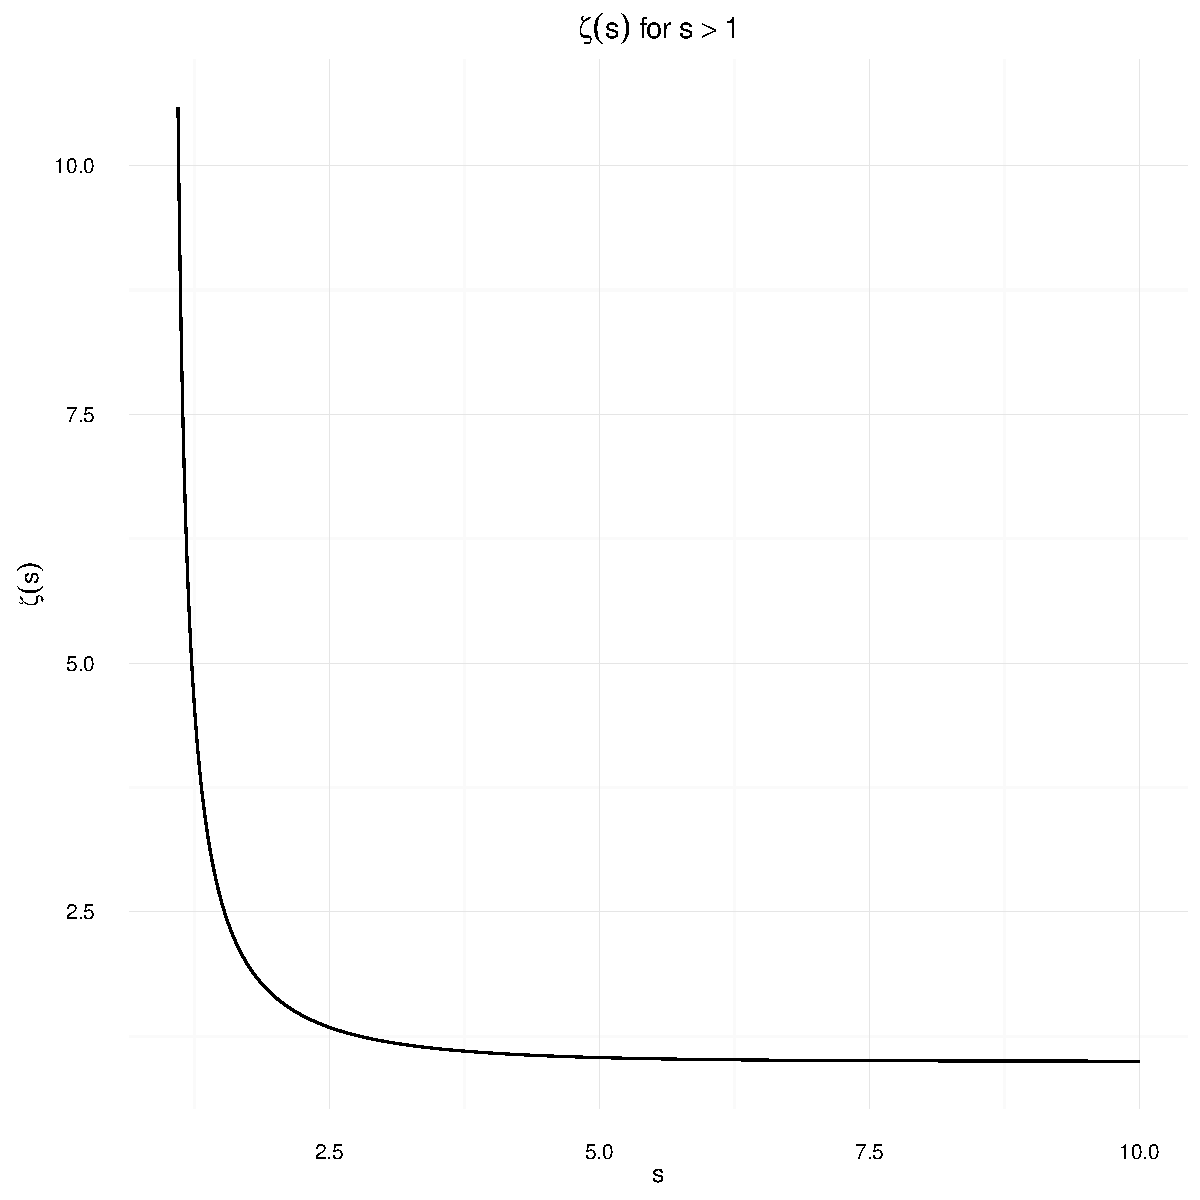
\includegraphics[width=0.5\textwidth]{zetagreater1.pdf}
  \end{frame}
  \begin{frame}{Riemann Zeta Function}
      \pause
      \begin{block}{Second definition}
          $$
          \zeta\left(s\right) = \sum_{n=1}^{\infty} \frac{1}{n^s} \qquad
          s \in \Complex; \Rpart{s} > 1
          $$
      \end{block}
      \pause
      \begin{block}{Third Definition}
          $\zeta(s)$ is the (unique) analytic continuation of the function in
          the second definition for all $s \ne 1$
      \end{block}
  \end{frame}
  \begin{frame}{Riemann Zeta Function}
      \pause
      \begin{block}{Fourth Definition}
          $$
          \zeta\left(s\right) = \product_{p \textrm{ prime}} \frac{1}{1 - p^{-s}}
          $$
      \end{block}
  \end{frame}
  \begin{frame}{Zeros}
      \pause
      \begin{block}{Trivial Zeros}
          $$
          \zeta(s) = 0 \quad \forall s \in \left\{-2, -4, -6, \ldots \right\}
          $$
      \end{block}
      \pause
      \begin{block}{Non-Trivial Zeros}
          So far, every non-trivial zero of $\zeta(s)$ which has been found
          lies on the line $\frac{1}{2} + it, t \in (-\infty, \infty)$.
      \end{block}
      \pause
      \begin{block}{Highly Non-Trivial Zeros}
          The statement of the problem is concerned with the existence of
          non-trivial zeros which do not lie on that line.
      \end{block}
  \end{frame}
  \begin{frame}{Consequences of the Riemann Hypothesis}
      \pause
      \begin{block}{Prime Number Theorem}
          Using RH we get a tight bound on the remainder term of the prime
          number theorem expression for the number of primes below $x$
          $$
          \pi(x) = \underbrace{\integral_{2}^{x} \frac{1}{\log t}
          dt}_{\eqqcolon Li(x)} + O(\sqrt{x}\log x)
          $$\pause
          In particular, RH implies
          $$
          \left| \pi(x) - Li(x) \right| < \frac{1}{8\pi}\sqrt{x}\log x \quad
          x \ge 2657
          $$
      \end{block}
  \end{frame}
  \begin{frame}{Consequences of the Riemann Hypothesis}
      \pause
      \begin{block}{Growth of the Divisor Function}
          Let $\sigma(n) = \sum_{d | n}d$. Then RH implies
          $$
          \sigma(n) < e^{\gamma} n \log\log n \quad n > 5040
          $$
      \end{block}
  \end{frame}

  \section{Navier-Stokes Existence and Smoothness}
  \begin{frame}{Navier-Stokes Existence and Smoothness}
      \begin{block}{Problem Statement}
          Prove that there exist smooth solutions with finite energy of the
          Navier-Stokes equations for any given divergence-free initial
          velocity field with no external force applied on either $\Real^3$
          or $\Real^3/\Integer$.\pause\\
          OR prove that there exists a divergence-free
          intial velocity field and a smooth external force which does not
          have a smooth solution with finite energy.
      \end{block}
  \end{frame}
  \begin{frame}{Navier-Stokes Equations}
      \pause
      \begin{block}{Material Derivative}
          We define $\frac{D}{Dt} \coloneqq \frac{\partial}{\partial t} +
          \mathbf{u} \cdot \nabla$
      \end{block}
      \pause
      \begin{block}{Incompressible Navier-Stokes}
          $$
          \frac{D \mathbf{u}}{D t} = -\nabla p + \nu\nabla^2\mathbf{u} +
          \mathbf{F}
          $$\pause
          $$
          \nabla \cdot \mathbf{u} = 0
          $$
      \end{block}
      \pause
      \begin{block}{Initial Conditions}
          $$
          \mathbf{u}(\mathbf{x}, 0) = \mathbf{u}^0(\mathbf{x}), \quad
          \mathbf{u}^0 \in C^{\infty},\; \nabla \cdot \mathbf{u}^0 = 0
          $$
      \end{block}
  \end{frame}
  \begin{frame}{Conditions Imposed}
      \linespread{0.8}
      \pause
      \begin{block}{Conditions Imposed on $\mathbf{u}^0$ and $\mathbf{F}$}
          We require:
          $$
          \left| \partial^{\boldsymbol{\alpha}}_{\mathbf{x}} \mathbf{u}^0
          \right| \le
          C_{\boldsymbol{\alpha}K} \left(1 + \left|\mathbf{x}\right|\right)^{-K} \quad
          \forall K > 0, \; \forall \boldsymbol{\alpha} \in \Natural_0^3, \;
          \forall \mathbf{x} \in \Real^3
          $$\pause
          \begin{multline*}
          \left| \partial^{\boldsymbol{\alpha}}_{\mathbf{x}}
          \partial^m_t \mathbf{F}
          \right| \le
          C_{\boldsymbol{\alpha}mK} \left(1 + \left|\mathbf{x}\right| +
          t\right)^{-K} \\
          \forall K > 0, \; \forall \boldsymbol{\alpha} \in \Natural_0^3, \;
          \forall m \in \Natural_0, \; \forall \mathbf{x} \in \Real^3, \;
          \forall t \in [0, \infty)
          \end{multline*}
      \end{block}
      \pause
      \begin{block}{Physically Reasonable Solutions}
          We require
          $$
          p, \mathbf{u} \in C^{\infty}(\Real^3 \times [0, \infty))
          $$
          \pause
          $$
          \integral_{\Real^n} \left| \mathbf{u}(\mathbf{x}, t) \right|^2
          d\mathbf{x} < C \quad \forall t \in [0, \infty)
          $$
      \end{block}
  \end{frame}
  \begin{frame}{Navier-Stokes Existence and Smoothness}
      \begin{block}{Problem Statement}
          Prove that there exist smooth solutions with finite energy of the
          Navier-Stokes equations for any given divergence-free initial
          velocity field with no external force applied on either $\Real^3$
          or $\Real^3/\Integer$.\pause\\
          OR prove that there exists a divergence-free
          intial velocity field and a smooth external force which does not
          have a smooth solution with finite energy.
      \end{block}
  \end{frame}

  \section{\Poincare{} Conjecture}
  \begin{frame}{\Poincare{} Conjecture}
      \begin{block}{Problem Statement}
          Prove that every simply connected, closed 3-manifold is
          homeomorphic to the 3-sphere.
      \end{block}
  \end{frame}
  \begin{frame}{Manifolds}
      \linespread{0.9}
      \pause
      \begin{block}{Topology}
          Given a set $X$, a \textit{topology} $\tau$ on $X$ is a collection of
          subsets of $X$ such that
          \begin{itemize}
              \item $X \in \tau, \emptyset \in \tau$
              \item The union of any collection of elements of $\tau$ is in
                  $\tau$
              \item The intersection of any \alert{finite} collection of
                  elements of $\tau$ is in $\tau$
          \end{itemize}
          The elements of $\tau$ are then called \textit{open sets}
      \end{block}
      \pause
      \begin{block}{Topological Field}
          A \textit{topological field} is a field which is also endowed with a
          topology.
      \end{block}
      \pause
      \begin{block}{Topological Vector Space}
          A \textit{topological vector space} is a vector space $X$ over a
          topological field $\mathbf{K}$ which is endowed with a topology such
          that vector addition and scalar multiplication are continuous
          functions.
      \end{block}
  \end{frame}
  \begin{frame}{Manifolds}
      \linespread{0.8}
      \pause
      \begin{block}{Homeomorphism}
          A \textit{homeomorphism} is a continuous function between two
          topological spaces whose inverse is continuous.
      \end{block}
      \pause
      \begin{block}{Manifolds}
          A \textit{manifold} $M$ is a topological space which is locally
          homeomorphic to a topological vector space.
      \end{block}
      \pause
      \begin{block}{Compact Manifold}
          A manifold $M$ is \textit{compact} if for every open cover there
          exists a finite subcover. That is
          \begin{multline*}
              \linespread{0.8}
          \forall \left\{U_a\right\}_{a \in A} \textrm{ s.t } \bigcup_{a\in A}
          U_a = M,
          U_a \textrm{ open}\\
          \exists J \subset A, |J| < \infty : \bigcup_{j \in J}U_j = M
          \end{multline*}
      \end{block}
  \end{frame}
  \begin{frame}{Manifolds}
      \linespread{0.8}
      \pause
      \begin{block}{Closed Manifold}
          A manifold is \textit{closed} if it is compact and does not contain
          its boundary
      \end{block}
      \pause
      \begin{block}{Path Connected}
          A manifold $M$ is \textit{path connected} if there exists a path
          connecting every two points in $M$
      \end{block}
      \pause
      \begin{block}{Simply Connected}
          Formally, a manifold $M$ is \textit{simply connected} if it is path
          connected and any two paths from $x \in M$ to $y \in M$ are
          homotopic relative to their endpoints
      \end{block}
      \pause
      \begin{block}{3-Manifold}
          A \textit{3-manifold} is a manifold which is locally homeomorphic to
          $\Real^3$
      \end{block}
      \pause
      \begin{block}{3-Sphere}
          $S^3 = \left\{\left(x_0, x_1, x_2, x_3) \in \Real^4 | x_0^2 + x_1^2 + x_2^2 +
          x_3^2 = 1\right\}$
      \end{block}
  \end{frame}
  \begin{frame}{\Poincare{} Conjecture}
      \begin{block}{Problem Statement}
          Prove that every simply connected, closed 3-manifold is
          homeomorphic to the 3-sphere.
      \end{block}
  \end{frame}

  \section{Pause}
  \begin{frame}{Questions}
      \begin{block}{}
          Any questions?
      \end{block}
  \end{frame}


  \section{Hodge Conjecture}
  \begin{frame}{Hodge Conjecture}
      \begin{block}{Problem Statement}
          Prove that on a projective non-singular algebraic variety over
          $\Complex$, any Hodge class is a rational linear combination of
          classes $cl(Z)$ of algebraic cycles.
          \note{This definition comes from the CMI}
      \end{block}
      % \begin{block}{Problem Statement}
      %     Let $X$ be a non-singular complex projective manifold. Then every
      %     Hodge class on $X$ is a linear combination with rational
      %     coefficients of the cohomology classes of complex subvarities of $X$.
      %     \note{This definition comes from wikipedia}
      % \end{block}
  \end{frame}
  \begin{frame}{Projective Algebraic Varieties over $\Complex$}
      \pause
      \begin{block}{Complex Projective Space}
          The \textit{complex projective space} of dimension $n$, denoted by
          $\CP^n$, is the set of all \alert{complex} lines in $\Complex^{n+1}$
          which pass through the origin.
      \end{block}
      \pause
      \begin{block}{Homogeneous Coordinates}
          We can identify each line in a complex projective space with a set of
          \textit{homogeneous coordinates}, usually denoted $[z_1 : z_2 :
          \cdots : z_{n+1}]$. These are unique up to scalar multiplication.
      \end{block}
      \pause
      \begin{block}{Homogeneous Polynomial}
          A \textit{homogeneous polynomial} is a polynomial whose non-zero
          terms have the same degree.
          \pause\\
          Important property: if $P(\vec{x})$ is homogeneous, then
          $$P(\lambda\vec{x}) = \lambda^d P(\vec{x})$$
      \end{block}
  \end{frame}
  \begin{frame}{Projective Algebraic Varieties over $\Complex$}
      \linespread{0.7}
      \pause
      \begin{block}{Ring}
          $(R, +, \cdot)$ is a \textit{ring} if:
      \begin{multicols}{2}
          \begin{itemize}
              \item $(R, +)$ is an abelian group
              \item $\cdot$ is associative in $R$
              \item $\cdot$ has an identity in $R$
              \item $\cdot$ is distributive over $+$
          \end{itemize}
      \end{multicols}
      \end{block}
      \pause
      \begin{block}{Ideal}
          Let $(R, +, \cdot)$ be a ring. Then $I \subseteq R$ is an \textit{ideal} if:
          \begin{multicols}{2}
              \begin{itemize}
                  \item $(I, +) \le (R, +)$
                  \item $\forall i \in I, \forall r \in R, \; i \cdot r, r
                      \cdot i \in I$
              \end{itemize}
          \end{multicols}
      \end{block}
      \pause
      \begin{block}{Prime Ideal}
          An ideal $(P, +, \cdot)$ with $P \subset R$ is a \textit{prime
          ideal} if
          $$a, b \in R, a\cdot b \in P \Rightarrow a \in P \textrm{ or
          } b \in P$$
      \end{block}
  \end{frame}
  \begin{frame}{Projective Algebraic Varieties over $\Complex$}
      \pause
      \begin{block}{Zero Locus}
          The \textit{zero locus} of a set of homogeneous polynomials $S$ in
          $\CP^n$ is defined to be $Z(S) = \left\{ x \in \CP^n | f(x) = 0
          \forall f \in S \right\}$
      \end{block}
      \pause
      \begin{block}{Projective Algebraic Variety}
          A \textit{projective algebraic variety} is a zero locus of a set of
          homogeneous polynomials which form a prime ideal
      \end{block}
  \end{frame}
  \begin{frame}{Singular Homology}
      \pause
      \begin{block}{$n$-Simplex}
          $$\Delta^n \coloneqq \left\{(t_0, \ldots, t_n) \in \Real^{n+1} | t_i
          \ge 0, \sum_{i=1}^n t_i = 1\right\}$$
      \end{block}
      \pause
      \begin{block}{Singular $n$-Simplex}
          A \textit{singular $n$-simplex} is a continuous map $\sigma_n:
          \Delta^n \rightarrow X$, where $X$ is a topological space
      \end{block}
      \pause
      \begin{block}{Boundary Operator}
          We denote the boundary of $\sigma_n(\Delta_n)$ by $\partial_n
          \sigma_n (\Delta_n)$ \pause \\
          Denote the group generated by the set of singular $n$-simplices by
          $C_n(X)$. It is a free Abelian group. \pause \\
          We can extend the boundary to the boundary operator $\partial_n : C_n
          \rightarrow C_{n-1}$ \pause \\
          It is a homomorphism
      \end{block}
  \end{frame}
  \begin{frame}{Singular Homology}
      \pause
      \begin{block}{Homology Group}
          We define the $i$th homology group
          $$\mathrm{Ker}(\partial_i)/\mathrm{Im}(\partial_{i+1})$$
          Its elements are known as homology classes.
      \end{block}
      \pause
      \begin{block}{Cohomology Group}
          \note{Don't worry how we get the duals}
          Consider the duals of $C_n(X)$, denoted $C^*_n(X)$ the corresponding
          dual homomorphisms $d_n : C^*_n(X) \rightarrow C^*_{n+1}(X)$ \pause
          \\
          We now define the $i$th cohomology group
          $$H^i(X) \coloneqq \mathrm{Ker}(d_i)/\mathrm{Im}(d_{i-1})$$
      \end{block}
  \end{frame}
  \begin{frame}{Hodge Class}
      \pause
      \begin{block}{Hodge Decomposition}
          A cohomology group $H^i(X)$ can be decomposed (under certain
          conditions) as follows:
          $$H^i(X) = \bigoplus_{p+q = i} H^{p,q}$$
          Where $H^{p,q}$ is the subgroup of cohomology classes which are
          represented by harmonic forms of type $(p,q)$
          \note{There is a connection between $d_n$ and the exterior
              derivatives defined later, we can use that to define the
          laplacian, then harmonic forms are defined from there}
      \end{block}
      \pause
      \begin{block}{Hodge Class}
          \note{The $\Rational$ comes from the Abelian group needed to define
              the dual}
          $$\mathrm{Hdg}^k(X) \coloneqq H^{2k}(X, \Rational) \cap H^{k,k}(X)$$
      \end{block}
  \end{frame}
  \begin{frame}{Algebraic Cycles}
      \linespread{0.8}
      \pause
      \begin{block}{Subvarities}
          A subvariety $Z$ of a variety $X$ is a subset of $X$ which is also a
          variety
      \end{block}
      \pause
      \begin{block}{Algebraic Cycle}
          An \textit{algebraic cycle} on a variety $X$ is a linear combination
          (with either integral of rational coefficients) of some set of
          subvarities $Z_i$, of the form
          $$\sum_i c_i Z_i$$
      \end{block}
      \pause
      \begin{block}{Cohomology Class of an Algebraic Cycle}
          The cohomology class of the above algebraic cycle is
          $$\sum_i c_i [Z_i]$$
          where $[Z_i]$ is the cohomology class of $Z_i$
      \end{block}
  \end{frame}
  \begin{frame}{Hodge Conjecture}
      \pause
      \begin{block}{Problem Statement}
          Prove that on a projective non-singular algebraic variety over
          $\Complex$, any Hodge class is a rational linear combination of
          classes $cl(Z)$ of algebraic cycles.
          \note{This definition comes from the CMI}
      \end{block}
  \end{frame}
  \section{Yang-Mills Existence and Mass Gap}
  \begin{frame}{Yang-Mills Existence and Mass Gap}
      \begin{block}{Problem Statement}
          Prove that for any compact simple gauge group $G$, a non-trivial
          quantum Yang-Mills theory exists on $\Real^4$ and has a mass gap
          $\Delta > 0$.
      \end{block}
  \end{frame}
  \begin{frame}{Disclaimer}
      \centering
      \alert{Imprecise definitions and notions ahead!}
  \end{frame}
  \begin{frame}{Yang-Mills Equations}
      \pause
      \begin{block}{Yang-Mills Equations}
          $$d_D F = 0$$
          $$*d_D * F = J$$
      \end{block}
      \pause
      \begin{block}{Setting}
          \begin{itemize}
              \item We are working on a general manifold \pause
              \item For the standard model, it's Minkowski space
          \end{itemize}
      \end{block}
  \end{frame}
  \begin{frame}{Manifolds and More}
      \linespread{0.7}
      \pause
      \begin{block}{Manifold}
          A manifold $M$ is a topological space which is locally homeomorphic
          to a topological vector space
      \end{block}
      \pause
      \begin{block}{Tangent Space}
          At each point $p \in M$ we associate a \textit{tangent space} 
          $T_p M$ of all vectors tangent to $p$. If $M$ is $n$-dimensional,
          then so is $T_p M$ for all $p \in M$.
      \end{block}
      \pause
      \begin{block}{Vector Field on Manifold}
          A \textit{vector field} on a manifold is a map which associates $p
          \in M$ to some $v \in T_p M$
      \end{block}
      \pause
      \begin{block}{Commutator of Vector Field}
          Given a vector-field $X$ on $M$, we define $X(p)$ to be the
          differential operator $\nabla_{v_p}$\pause \\
          \note{Yes, this is a conflation of notation}
          \note{$v_p$ is the element of $T_p M$ which is associated to $p$ by
          $X$}
          Given vector-fields $X, Y$ on $M$, we define
          $$[X, Y] \coloneqq X\circ Y - Y \circ X$$
      \note{This is a first-order differential operator}
      \end{block}
  \end{frame}
  \begin{frame}{Manifolds and More}
      \pause
      \begin{block}{Basis Vectors of $T_p M$}
          We denote the basis vectors of $T_p M$ by $\partial_i \equiv
          \underbrace{(0, \ldots, 1, \ldots, 0)}_{\text{1 in the $i$th place}}$
          \note{Make a point of the connection between this and the
          standard differential operators}
      \end{block}
      \pause
      \begin{block}{Cotangent Space}
          Associate with each $T_p M$ the dual of that vector space, denoted
          $T^*_p M$ which is the set of linear maps from $T_p M$ to $\Real$
      \end{block}
      \pause
      \begin{block}{Basis of Cotangent Space}
          $$\left\{ dx_j \right\}_j, \quad dx_j(\partial_k) \coloneqq
          \delta_{jk}$$
      \end{block}
      \pause
      \begin{block}{One-Forms}
          A \textit{one-form} $\omega$ associates each $p \in M$ with an
          element of $T^*_p M$
      \end{block}
  \end{frame}
  \begin{frame}{$p$-Forms}
      \pause
      \begin{block}{Tensor Product}
          For vectors $v, w$ belong to a vector space $V$, $v
          \otimes w = wv^{\mathrm{T}}$\pause\\
          This can be generalised to arbitrary tensors (\alert{don't ask})
      \end{block}
      \pause
      \begin{block}{Wedge Product}
          For vectors $v_1, v_2 \in V$, $$v_1 \wedge v_2 \coloneqq \frac{v_1
          \otimes v_2 - v_2 \otimes v_1}{2}$$ \pause \\
          For vectors $v_1, \ldots, v_n \in V$, $$v_1 \wedge \cdots \wedge v_n
          \coloneqq \frac{\sum_{\pi} \mathrm{sgn}(\pi) v_{\pi(1)} \otimes
          \cdots \otimes v_{\pi(n)}}{n!}$$
          where $\pi$ are permutations.
      \end{block}
  \end{frame}
  \begin{frame}{$p$-Forms}
      \pause
      \begin{block}{$p$th exterior product}
          For a vector space $V$, the \textit{$p$th exterior product} of $V$ is
          $\Lambda^p(V)$ which is spanned by vectors of the form $v_1 \wedge
          \cdots \wedge v_p$ \pause \\
          By convention, $\Lambda^0(V) \coloneqq \Real$
      \end{block}
      \pause
      \begin{block}{$p$-Forms}
          A $p$-form is a map $\omega$ which associates to each $p \in M$ an
          element of $\Lambda^p(T_p^* M)$ \pause \\
          $\Omega^p (M)$ denotes the set of all $p$-forms on $M$
      \end{block}
  \end{frame}
  \begin{frame}{Exterior Derivative}
      \linespread{0.7}
      \pause
      \begin{block}{Exterior Derivative Rough Idea}
          Usual definition of derivative
          $$\lim_{h \rightarrow 0}\frac{f(x + hy) - f(x)}{h}$$ \pause \\
          $f(x + hy)$ lives in $T_{x + hy}$ and $f(x)$ in $T_x$ \pause \\
          We can ``identify'' $T_{x+hy}$ with $T_x$ in some way and compute the
          derivative
      \end{block}
      \pause
      \begin{block}{Rules for Exterior Derivative}
          Exterior derivative maps $p$-form $\omega \in \Omega^p(M)$ to
          $(p+1)$-form $d\omega \in \Omega^{p+1}(M)$ \pause \\
          Exterior derivative is linear \pause \\
          $d(\alpha \wedge \beta) = d\alpha \wedge \beta + (-1)^p \alpha \wedge
          \beta$ \pause \\
          $d(d\omega) = 0$ \pause \\
          If $f$ is a scalar field (i.e. a 0-form) then $df = \sum_j
          (\partial_j f)dx_j$ \pause \\
          $d(f\omega) = df \wedge \omega + f d\omega$ for all 0-form $f$
      \end{block}
  \end{frame}
  \begin{frame}{Covariant Derivative or \textit{Connection}}
      \begin{block}{Covariant Derivative Rough Idea}
          Consider a notion of moving a tangent vector $v$ at a point $p$ in
          $M$ to a tangent vector $v'$ at another point $p'$ in $M$, whilst
          keeping them the same. \pause \\
          \note{$w$ is the direction we move in, we want to keep the
              components of the tangent vector the same.}
          $$\sum_j w_j (\partial_j v_k) = 0$$ \pause \\
          This requires a local coordinate system, we want it to work in any
          \pause \\
          \note{$A_l$ are Christoffel symbols, term from change of local
          coordinates}
          $$\sum_l w_l(\partial_l v + A_l v) = 0$$ \pause \\
          Define $$D_w v = \sum_l w_l ( \partial_l v + A_l v)$$
      \end{block}
  \end{frame}
  \begin{frame}{Vector Bundles}
      \pause
      \begin{block}{Vector Bundle}
          More generally, we can associate a vector space to each point in the
          manifold. Denote it $V_p$ and we call it a fibre. $M$ plus the $V_p$s
          are called a vector bundle. (All fibres must have the same dimension)
          \note{Link this back to the tangent space}
      \end{block}
      \pause
      \begin{block}{Sections}
          A \textit{section} is a map $s$ which associates an element of $V_p$
          to each $p \in M$
          \note{Give temperature example -- fibres are all $\Real$, section
          associates one of those values to each point in $M$}
      \end{block}
      \pause
      \begin{block}{Covariant Derivative}
          We can extend the covariant derivative to work on arbitrary sections
          in an analogous way
      \end{block}
  \end{frame}
  \begin{frame}{Gauge Theory}
      \pause
      \begin{block}{G-Bundle}
          Given a group $G$ and a \textit{representation} of it $V$, define a
          bundle over a manifold $M$ where each fibre is $V$.
      \end{block}
      \pause
      \begin{block}{Sections of a G-Bundle}
          A section of this G-bundle assigns to each $p \in M$ a group element
          $g(p)$ acting on $V$.
      \end{block}
      \pause
      \begin{block}{Gauge Symmetries and Groups}
          We call $g$ a \textit{gauge transformation} or \textit{gauge
          symmetry} and $G$ the \textit{gauge group}.
      \end{block}
  \end{frame}
  \begin{frame}{Final Steps}
      \pause
      \begin{block}{Curvature}
          Given a covariant derivative, we define the curvature
          $$F(v, w)s \coloneqq D_vD_ws - D_wD_vs - D_{[v, w]}s$$ \pause \\
          Note that $v, w$ are vector fields and $s$ is a section. $F(v, w)$
          takes a section and returns another section.
      \end{block}
      \pause
      \begin{block}{Exterior Covariant Derivative}
          Given a covariant derivative, you can define the exterior covariant
          derivative, in analogy to the exterior derivative. Denote it $d_D$
      \end{block}
  \end{frame}
  \begin{frame}{Final Steps}
      \pause
      \begin{block}{Hodge $*$-Product}
          Given a vector space $V$ with orthonormal basis ${e_1, \ldots, e_n}$
          $$*(e_{j_1} \wedge \cdots \wedge e_{j_p}) \coloneqq \mathrm{sgn}(j)
          e_{j_{p+1}} \wedge \cdots \wedge e_{j_n}$$ \pause \\
          Extend this definition linearly to all of $\Lambda^p(V)$. \pause \\
          This is then extended to any $p$-form $\omega \in \Omega^p(M)$.
      \end{block}
      \pause
      \begin{block}{Quantizing}
          Once you've fixed a gauge group $G$ and your connection (aka
          covariant derivative), you can construct a Yang-Mills theory\pause\\
          However, it still needs to be quantised, which is not necessarily
          easy.
      \end{block}
  \end{frame}
  \begin{frame}{Yang-Mills Equations}
      \pause
      \begin{block}{Yang-Mills Equations}
          $$d_D F = 0$$
          $$*d_D * F = J$$
      \end{block}
  \end{frame}
  \begin{frame}{Yang-Mills Existence and Mass Gap}
      \begin{block}{Problem Statement}
          Prove that for any compact simple gauge group $G$, a non-trivial
          quantum Yang-Mills theory exists on $\Real^4$ and has a mass gap
          $\Delta > 0$.
      \end{block}
  \end{frame}

  \section{Birch and Swinnerton-Dyer Conjecture}
  \begin{frame}{Birch and Swinnerton-Dyer Conjecture}
      \begin{block}{Problem Statement}
          Prove that the Taylor expansion at $s=1$ of the incomplete
          $L$-function $L(C, s)$ of a non-singular projective model $C$ of a
          curve $C_0$ defined by $f(x, y) = 0$ for a polynomial
          $f \in \Rational [x, y]$ has the form
          $c(s-1)^r + \text{higher order terms}$ with
          $r = \mathrm{rank}(C(\Rational))$.
      \end{block}
  \end{frame}
  \begin{frame}{Curves}
      \pause
      \begin{block}{Algebraic Curve}
          An \textit{algebraic curve} is a curve $C_0$ defined by the zeros
          of a polynomial in two variables $p(x, y)$
          \note{Give example of circle}
      \end{block}
      \pause
      \begin{block}{Plane Projective Curves}
          Given an algebraic curve, we can define it's corresponding plane
          projection $C$ in the projective plane ($\RP{} ^2$).
          $$p^h(x, y, z) \coloneqq z^{\mathrm{deg}(p)}p(\frac{x}{z},
          \frac{y}{z})$$
      \end{block}
      \pause
      \begin{block}{Rational Solutions}
          If $p(x, y) \in \Rational\left[x, y\right]$, then we can look at the
          zeros in $\Rational$, denoted by $C_0(\Rational)$ (and
          correspondingly, zeros of $p^h$ in $\Rational$ denoted by
          $C(\Rational)$)
      \end{block}
  \end{frame}
  \begin{frame}{Characterising Curves}
      \pause
      \begin{block}{Number of Solutions}
          Either $C_0(\Rational)$ and $C(\Rational)$ are finite, or they are
          both infinite
      \end{block}
      \pause
      \begin{block}{Genus of Curves}
          Plane projective curves $C$ can be characterized by their
          \textit{genus} \note{think number of holes}, and we call the genus of
          $C$ the genus of $C_0$ too \pause \\
          There are results about the size of $C_0(\Rational)$ for genus $\ge
          2$ and $0$, but genus $1$ remains open in general
      \end{block}
  \end{frame}
  \begin{frame}{Group Structure}
      \pause
      \begin{block}{Elliptic Curves}
          If $C$ is non-singular and has a rational point, then it is called an
          \textit{elliptic curve over $\Rational$}
      \end{block}
      \pause
      \begin{block}{Mordell-Weil Theorem}
          An elliptic curve $C$ over $\Rational$ defines a group $C(\Rational)$
          which satisfies 
          $$C(\Rational) \simeq \Integer^r
          \oplus C(\Rational)^{\mathrm{tors}}$$
          \pause
          We call $r \in \Natural_0$ the rank of $C$.
          $C(\Rational)^{\mathrm{tors}}$ is some finite Abelian group. \pause
          \\
          $$r = 0 \iff \left|C(\Rational)\right| < \infty$$
      \end{block}
  \end{frame}
  \begin{frame}{Incomplete $L$-Series}
      \pause
      \begin{block}{Necessaries}
          An elliptic curve over $\Rational$ can be written in the form
          $$y^2 = x^3 + ax + b$$
          \pause
          $\Delta \coloneqq -16(4a^3 + 27b^2)$ \pause \\
          $N_p \coloneqq \left|\left\{\text{solutions of } y^2 = x^3 + ax + b
          \text{ mod } p\right\}\right|$ \pause \\
          $a_p \coloneqq N_p - p$
      \end{block}
      \pause
      \begin{block}{Incomplete $L$-Series of $C$}
          $$L(C, s) \coloneqq \product_{p\; \nmid\; 2 \Delta} \left(1 -
              a_p p^{-s} + p^{1 - 2s}\right)^{-1}$$
          For primes $p$. This converges for $\Rpart{s} > 3/2$ and can be
          continued analytically to the whole of $\Complex$ 
      \end{block}
  \end{frame}
  \begin{frame}{Birch and Swinnerton-Dyer Conjecture}
      \pause
      \begin{block}{Problem Statement}
          Prove that the Taylor expansion at $s=1$ of $L(C, s)$ has the form
          $$c(s-1)^r + \text{higher order terms}$$ with $c \ne 0$ and $r =
          \mathrm{rank}(C(\Rational))$
      \end{block}
      \pause
      \begin{block}{A Consequence}
          $L(C, 1) = 0 \iff C(\Rational)$ is infinite
      \end{block}
  \end{frame}
  \section{Finish}
  \begin{frame}{Questions}
      Any questions?
  \end{frame}



\end{document}
